\documentclass[11pt]{article}
\usepackage[margin=1in]{geometry}
\usepackage{graphicx}
\usepackage{amsmath}
\usepackage{amssymb}
\usepackage{float}
\usepackage{subcaption}
\usepackage{booktabs}

\title{Meeting Document}

\begin{document}
\maketitle

\section{$c_d$ Estimation}
  For the $c_d$ estimation, we first top code the sentences observed in the data to 720 months, following the convention of Hester 2017. This only affects $0.004$ of all cases (82/17,516). We then use this top coded sentence to compute each $\tau_i$. We also use our data to compute $\theta_i$ for each defendant. We use these two quantities, along with the top coded sentence variable, to create the convex hull for the judges. Once we have the convex hull for each judge, we use it to compute $l_j(\theta_i \tau_i)$ and $u_j(\theta_i \tau_i)$ for each defendant. We then use this information to split the defendants into three groups as specified by the write up. We calculate the overall negative log likelihood (i.e. we sum the negative log likelihood of each individual defendant) and then minimize this quantity using a black box optimizer. We add $\epsilon=0.0001$ to each likelihood before taking the log to avoid taking the log of 0. The optimization algorithm is sensitive to the initialization and to the value of $\epsilon$. There are some initializations and values of $\epsilon$ for which the algorithm won't terminate successfully, and it will return the message "Desired error not necessarily achieved due to precision loss". The table below contains some results.

  \begin{table}[H]
  \centering
  \caption{Estimation Results}
  \label{tab:my-table}
  \begin{tabular}{|l|l|l|l|}
  \hline
  \textbf{$(\mu_0,\sigma_0)$} & \textbf{$\epsilon$} & \textbf{$(\mu^*,\sigma^*)$} & \textbf{Success} \\ \hline
  8,8   & 0.00001 & -28.8, 46.6 & False \\ \hline
  8,8   & 0.0001  & -27.8, 38.4 & True  \\ \hline
  8,8   & 0.001   & -26.3, 31.6 & True  \\ \hline
  10,10 & 0.001   & -26.3, 31.6 & True  \\ \hline
  10,10 & 0.0001  & -27.8, 39.1 & True  \\ \hline
  10,8  & 0.0001  & -27.8, 39.1 & True  \\ \hline
  10,5  & 0.0001  & -27.8, 39.1 & True  \\ \hline
  \end{tabular}
  \end{table}

\section{Overview}
  This document contains bar charts of the number of GS judge days each judge was assigned to work each week. Here, I am only including assignments to counties. So assignments of the type "administrative week" or "6th circuit court" are excluded. The document also contains the number of judge days each county was assigned each week in our data. The observations are listed chronologically, so week 1 in our data is mid July 2000 and week 52 is mid July 2001.

\section{Weekly Judge Days by County}
  \begin{figure}[H]
    \centering
    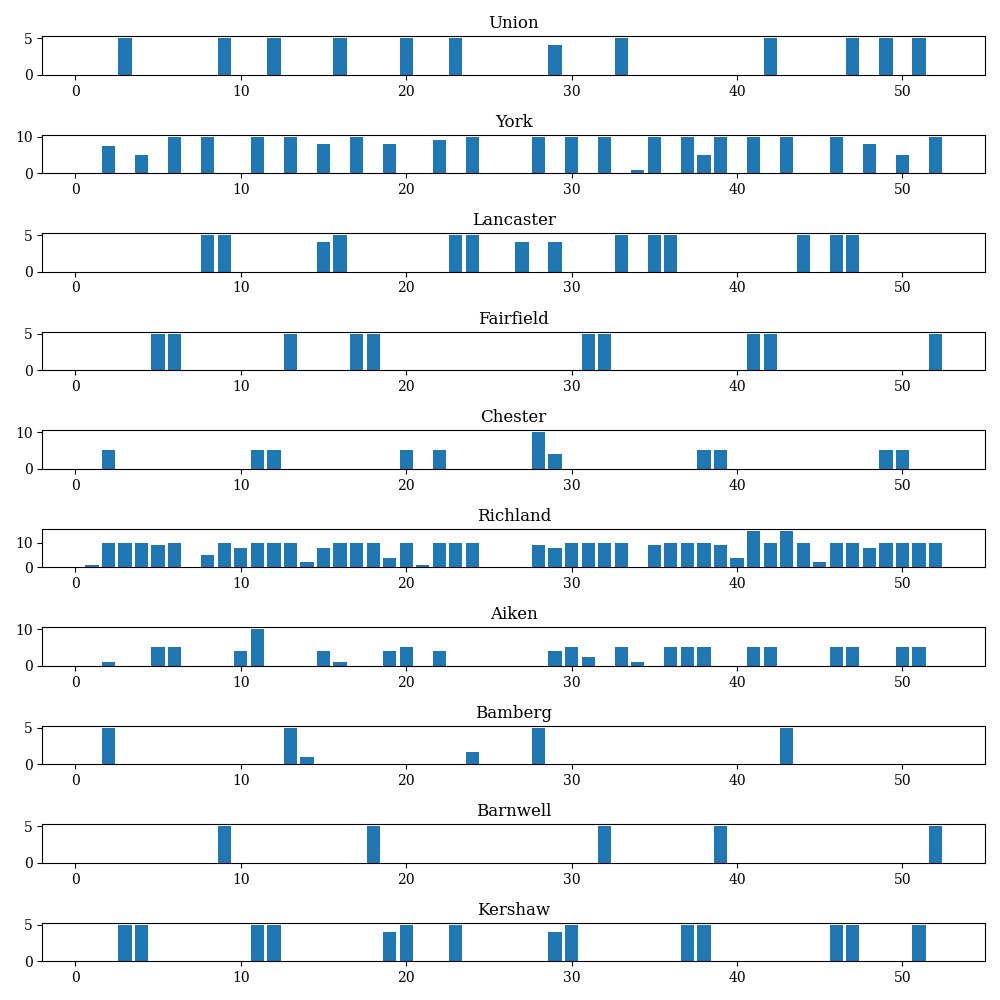
\includegraphics[width=\textwidth]{../../../output/figures/Exploration/County_weekly_judge_days_0}
  \end{figure}

  \begin{figure}[H]
    \centering
    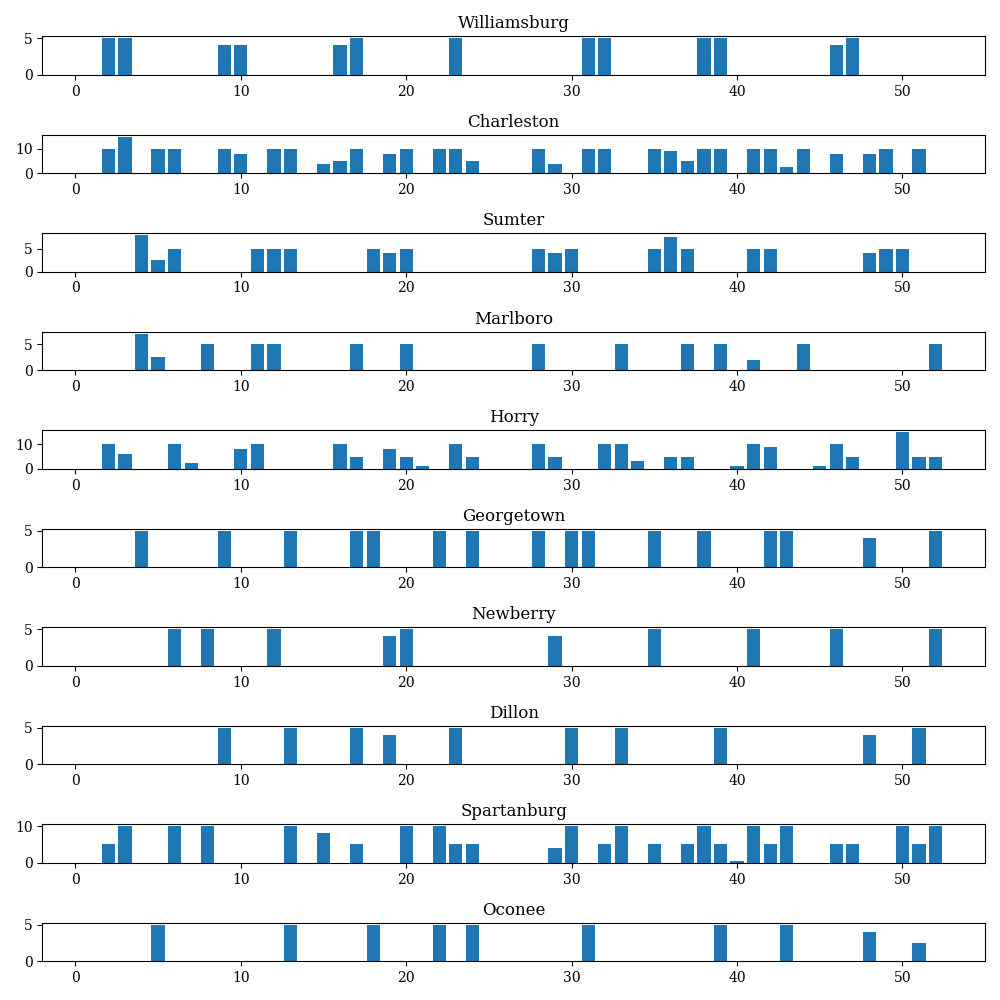
\includegraphics[width=\textwidth]{../../../output/figures/Exploration/County_weekly_judge_days_1}
  \end{figure}

  \begin{figure}[H]
    \centering
    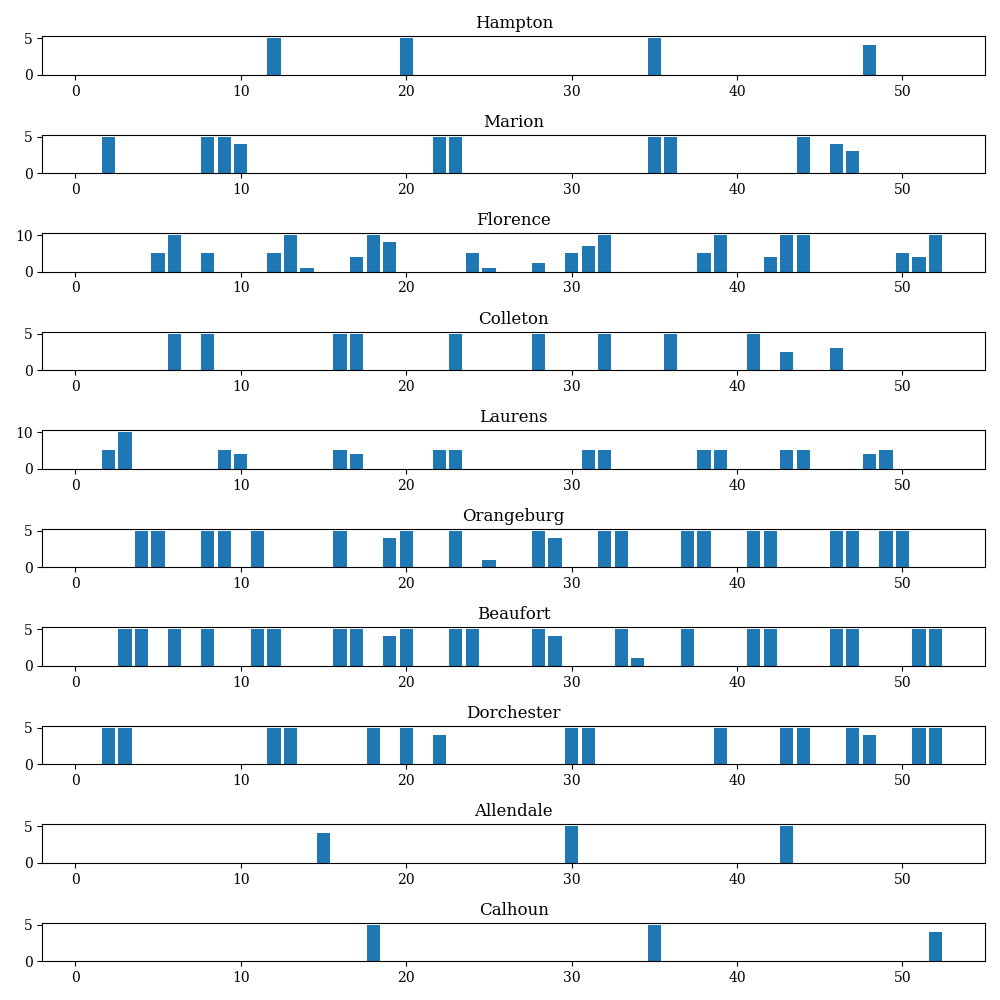
\includegraphics[width=\textwidth]{../../../output/figures/Exploration/County_weekly_judge_days_2}
  \end{figure}

  \begin{figure}[H]
    \centering
    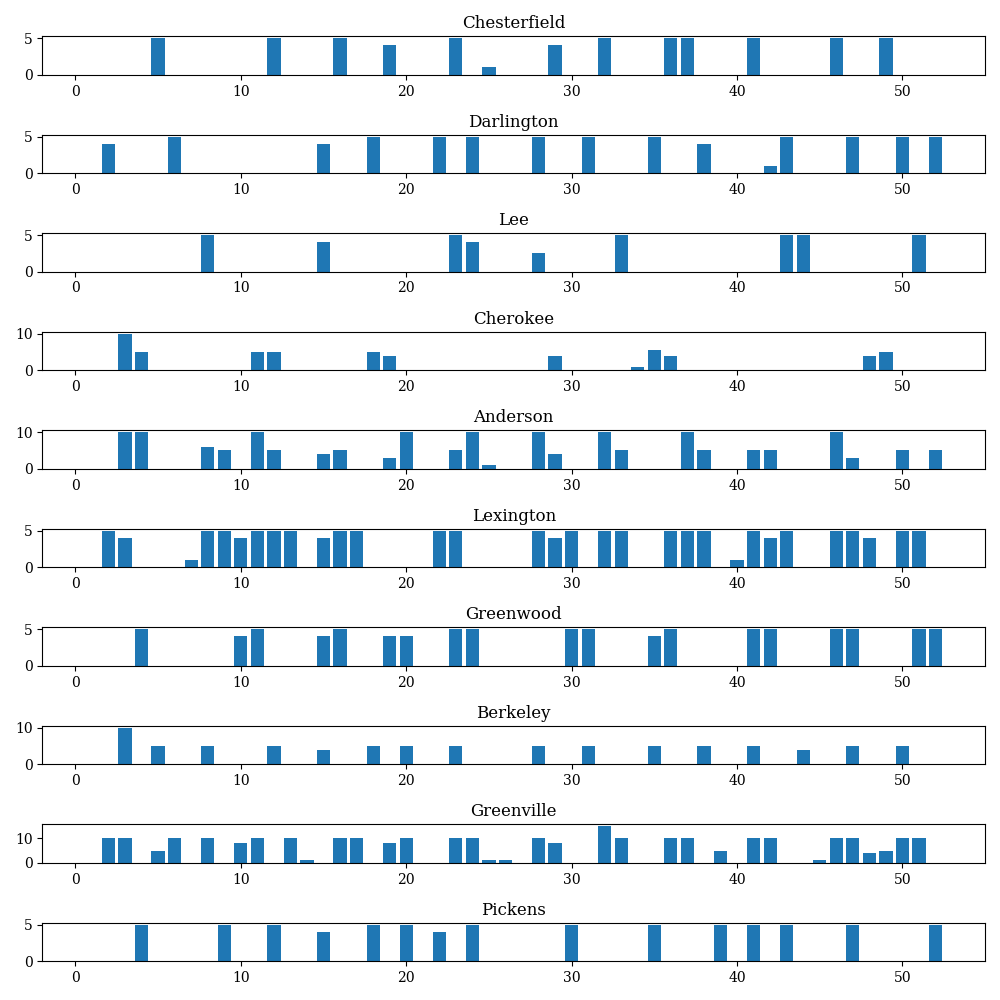
\includegraphics[width=\textwidth]{../../../output/figures/Exploration/County_weekly_judge_days_3}
  \end{figure}

  \begin{figure}[H]
    \centering
    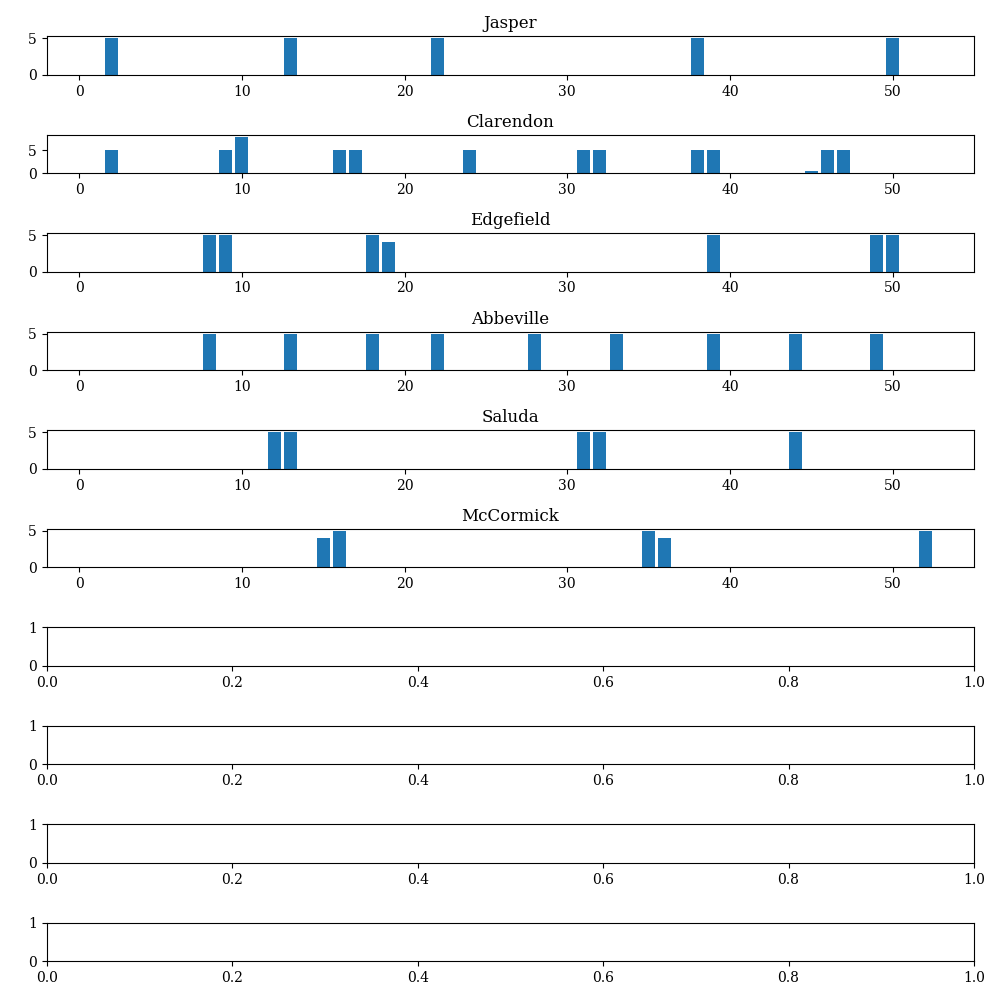
\includegraphics[width=\textwidth]{../../../output/figures/Exploration/County_weekly_judge_days_4}
  \end{figure}

\section{Weekly Judge Days by Judge}
  \begin{figure}[H]
    \centering
    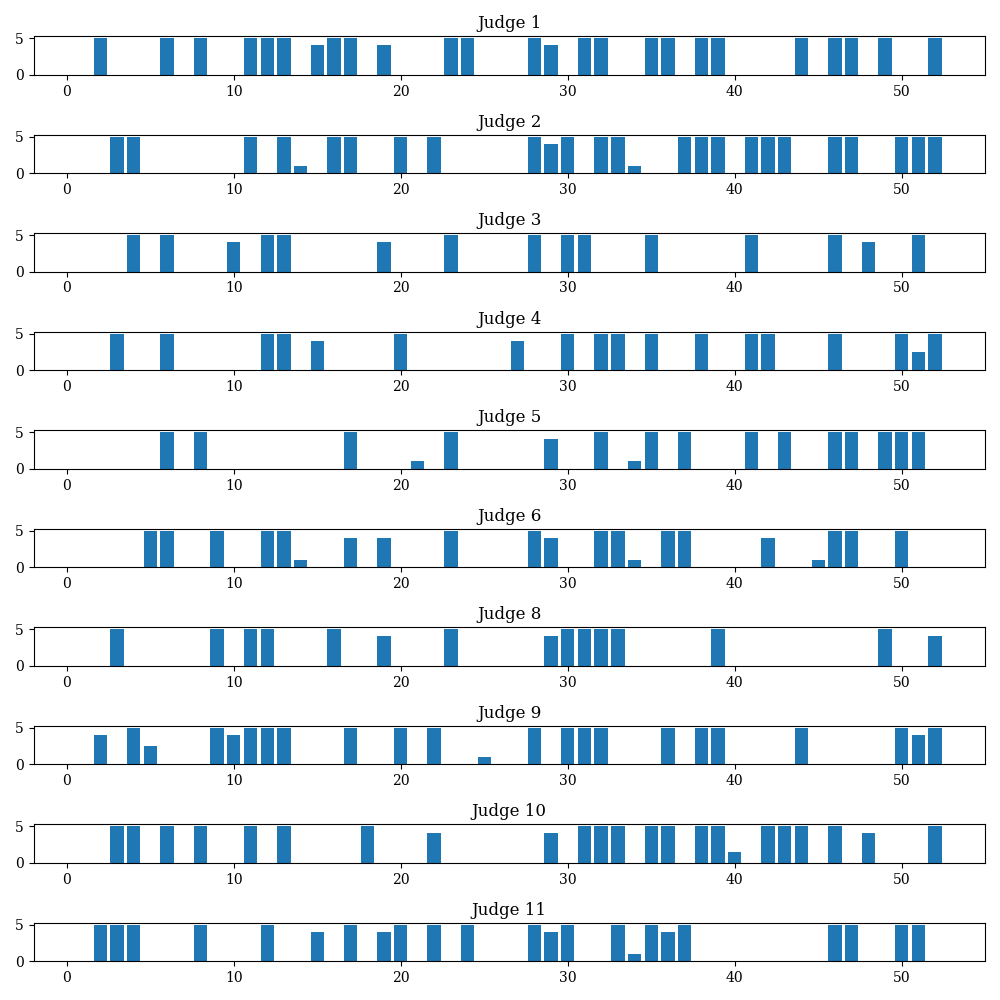
\includegraphics[width=\textwidth]{../../../output/figures/Exploration/JudgeID_weekly_judge_days_0}
  \end{figure}

  \begin{figure}[H]
    \centering
    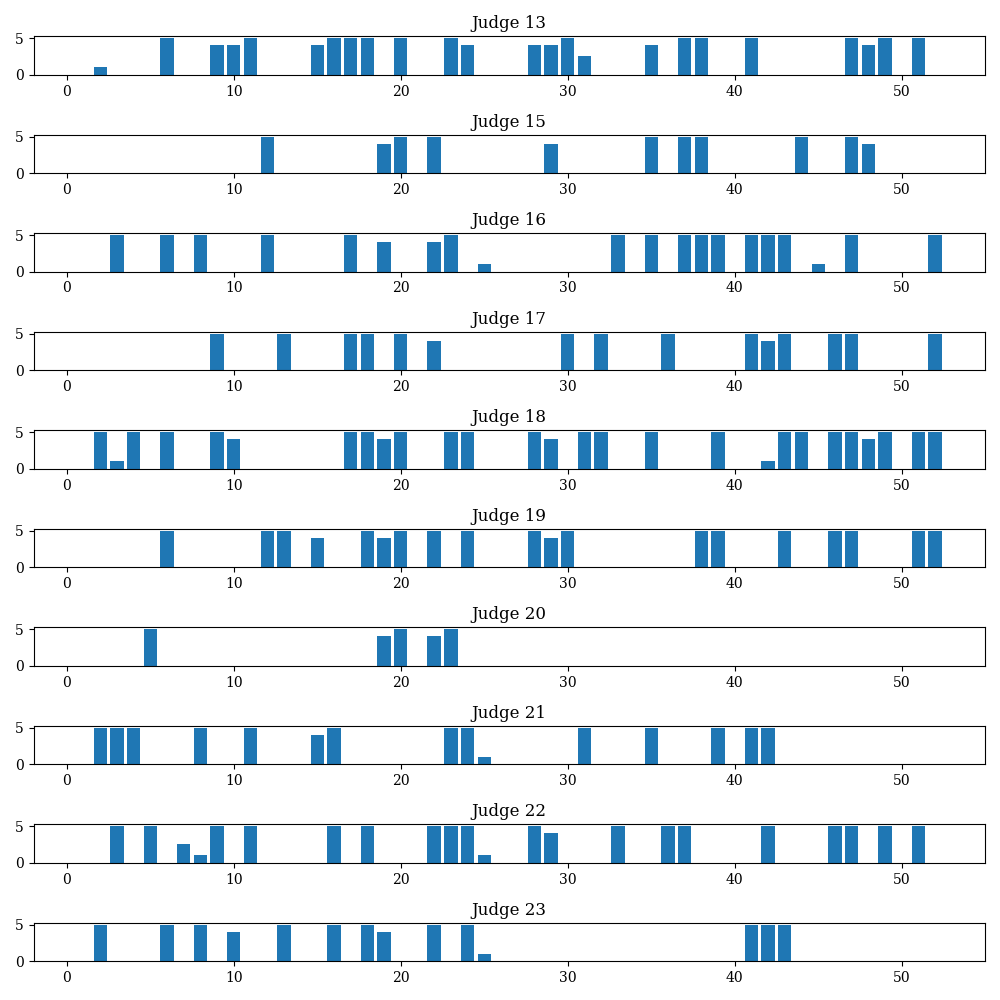
\includegraphics[width=\textwidth]{../../../output/figures/Exploration/JudgeID_weekly_judge_days_1}
  \end{figure}

  \begin{figure}[H]
    \centering
    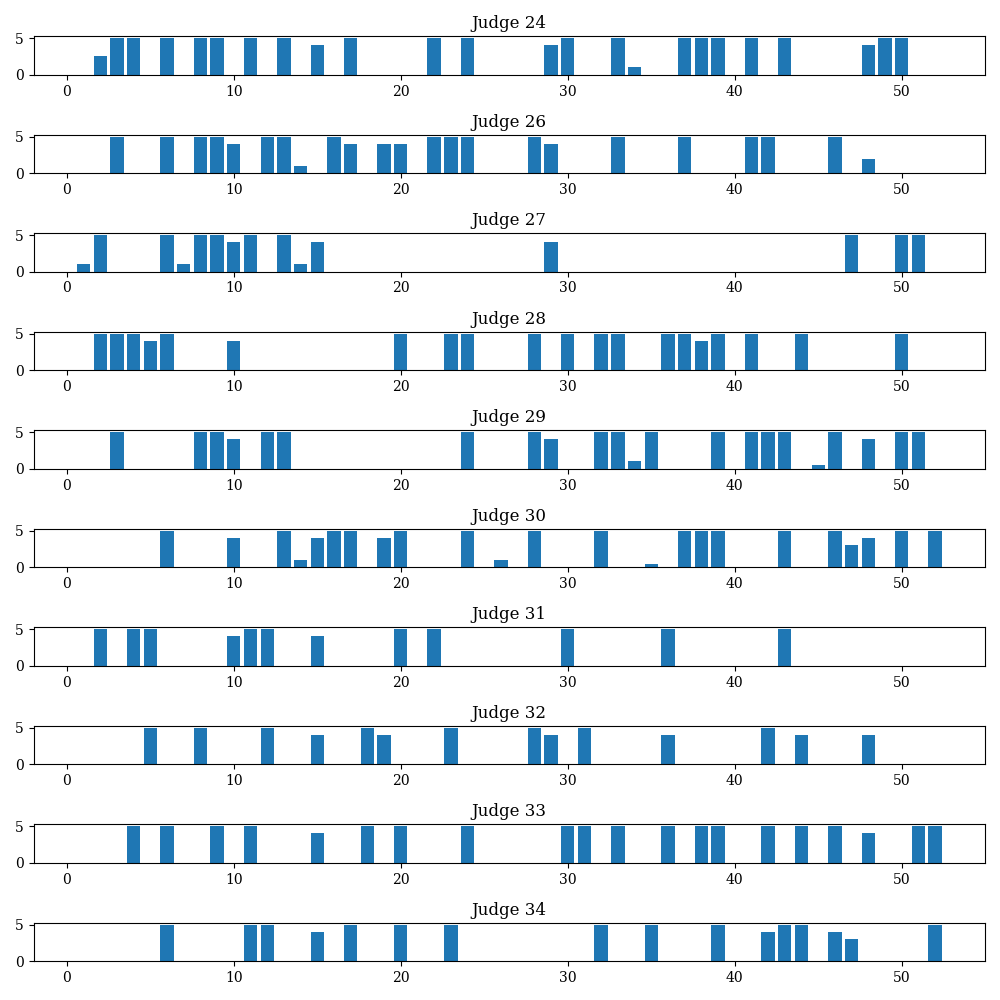
\includegraphics[width=\textwidth]{../../../output/figures/Exploration/JudgeID_weekly_judge_days_2}
  \end{figure}

  \begin{figure}[H]
    \centering
    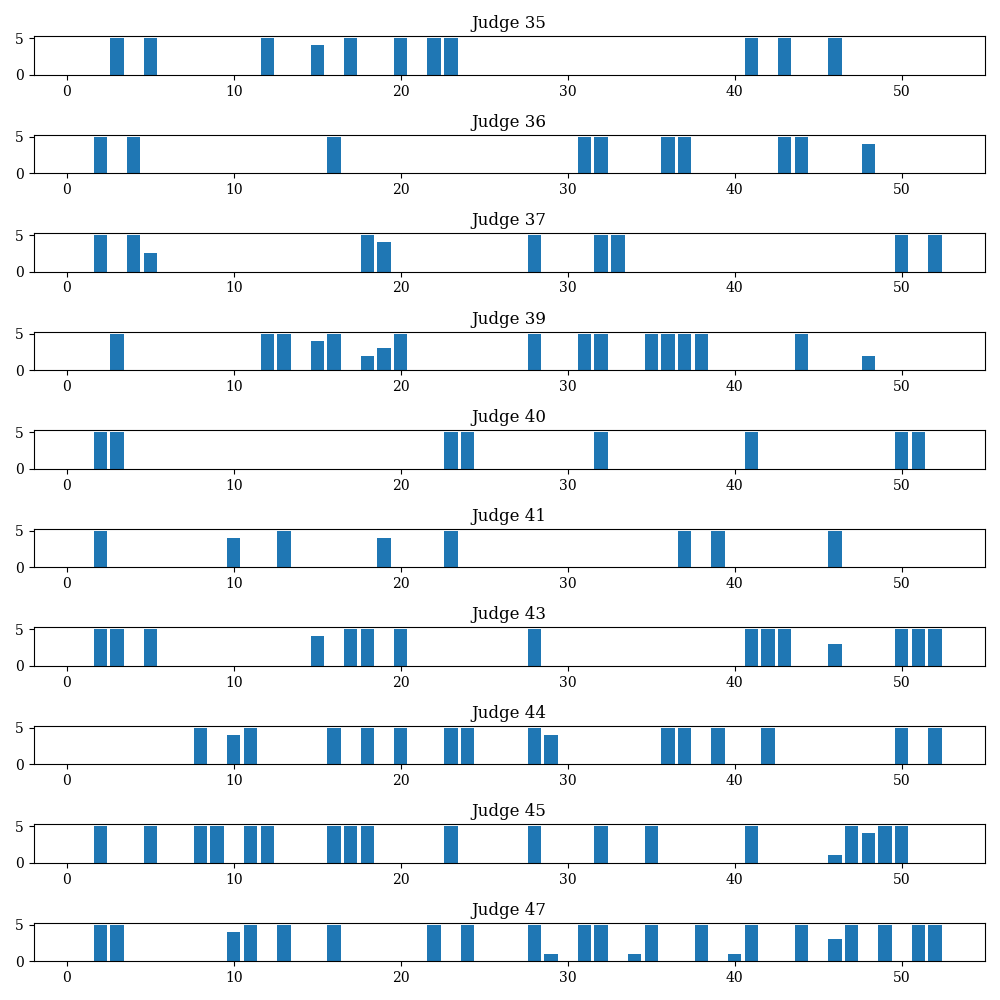
\includegraphics[width=\textwidth]{../../../output/figures/Exploration/JudgeID_weekly_judge_days_3}
  \end{figure}

  \begin{figure}[H]
    \centering
    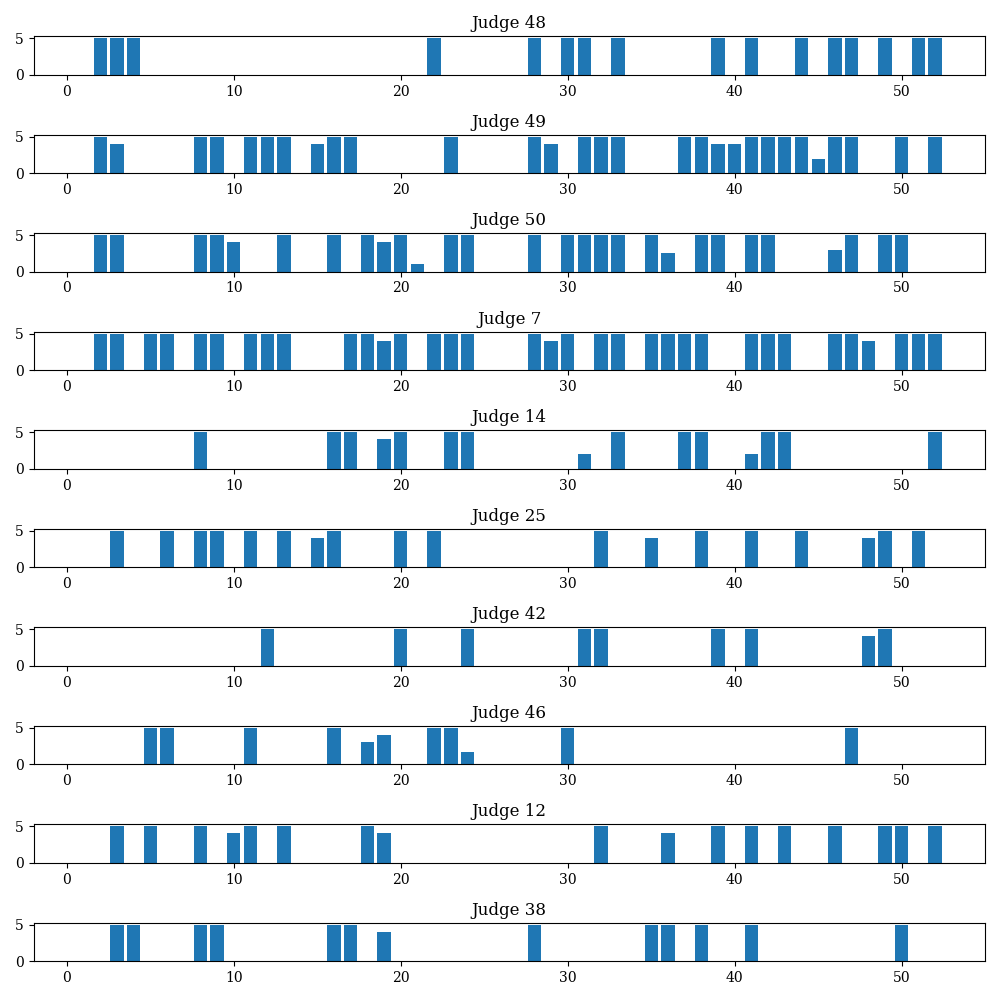
\includegraphics[width=\textwidth]{../../../output/figures/Exploration/JudgeID_weekly_judge_days_4}
  \end{figure}


\end{document}
